\section{Modeling An Election Algorithm as a Stationary Markov Chain}

%State how sequences are generated.
%State how transition probabilities are generated in the profile chain. State what the profile chain could be used for when collected.

% 3 sections
% Execution assumptions
% algorithmic changes
% producing the profile chain

\subsection{Execution Environment}

Execution occurs in a real-time synchronized environment.
Processes synchronize their clocks and execute steps of the election algorithm at predefined intervals.
Processes with clocks that are not sufficiently synchronized cannot form groups.
For this work, process execution occurs in an environment where the clocks are sufficiently synchronized to consistently form groups.

The execution environment is subject to omission failures.
In an omission failure, a message sent by one process to another process is lost in transit.
Omission failures can occur for many reasons.
Network congestion is a typical culprit.
Routers may drop packets or delay their delivery when there is a large amount of traffic or a network issue.
In a real-time environment, packets that are delayed to miss real-time deadlines will have the same appearance as a dropped packet.
The execution environment for the election algorithm has a omission failure occurrence modeled as a Bernoulli trial.
In this model, each message has some probability $p$ of being delivered within the timing constraints imposed by the real-time schedule.
For the purpose of analyzing the effects of omission failures, processes are not subject to other faults.
A process will not crash or halt during execution.

\subsection{Election Algorithm}

The original Garcia-Molina algorithm has been modified so the observations of the coordinator process have the Markov property.
The full algorithm is presented below.
The rest of this section describes the changes that were made to the algorithm and shows how the combination of those changes allow the observations of the coordinator to be modeled as a Markov process.
The execution model of this algorithm assumes a real-time system using a round-robin scheduler.
At a predetermined time and following predetermined intervals the algorithm executes at each process.
Using the synchronized clocks, all processes execute either $Check()$ or $Timeout()$ at the same time.
Processes can only form groups if their clocks are sufficiently in sync with another process' clock.

\begin{algorithmic}

\State $AllPeers \gets \{ 1, 2, ..., N \}$
\State $Coordinators \gets \emptyset$
\State $UpPeers \gets { Me }$
\State $State \gets Normal$
\State $Coordinator \gets Me$
\State $Responses \gets \emptyset$
\State $Counter \gets$ A random initial identifier
\State $GroupID \gets (Me,Counter)$

\State

\Function{Check}{}
    \State This function is called at the start of a round by the leader
    \If {$State = Normal$ and $Coordinator \gets Me$}
        \State $Responses \gets \emptyset$
        \State $TempSet \gets \emptyset$
        \For {$j = (AllPeers - \{Me\})$}
            \State $AreYouCoordinator(j)$
            \State $TempSet \gets TempSet \cup j$
        \EndFor
        \State Peers which respond "Yes" to $AreYouCoordinator$ are put into the $Responses$ set.
        \State When an $AreYouThere$ response is "No" and this process is a coordinator, the querying process is put in the $Responses$ set.
        \State Wait for $Timeout(CheckTimeout)$, Peers that do not respond are removed from UpPeers.
        \State $UpPeers \gets (TempSet-Responses) \cup {Me}$
        \If {$Responses = \emptyset$}
            \Return
        \EndIf
        \State $p \gets \max(Responses)$
        \If $Me > p$
            \State Wait time proportional to me-p
        \EndIf
        \Call{Merge}{Responses}
    \EndIf
    \State The next call to this is after Timeout(CheckTimeout)
\EndFunction

\State

\Function{Timeout}{}
    \State This function is called at the start of a round by the group members
    \If {$Coordinator = Me$}
        \Return
    \Else
        \Call{AreYouThere}{Coordinator,GroupID,Me}
        \If{Response is No}
            \Call{Recovery}{}
        \EndIf
    \EndIf
    \State The next call to this is after Timeout(TimeoutTimeout)
\EndFunction

\State

\Function{Merge}{Coordinators}
    \State This function invites all coordinators in Coordinators to join a group led by Me
    \State $State \gets Election$
    \State Stop work
    \State $Counter \gets Counter+1$
    \State $GroupID \gets (Me,Counter)$
    \State $Coordinator \gets Me$
    \State $TempSet \gets UpPeers - {Me}$
    \State $UpPeers \gets \emptyset$
    \For {$j \in Coordinators$}
        \Call{Invite}{j,Coordinator,GroupID}
    \EndFor
    \For {$j \in TempSet$}
        \Call{Invite}{j,Coordinator,GroupID}
    \EndFor
    \State Wait for $Timeout(InviteTimeout)$, Peers that accept the invite are added to UpPeers
    \State $State \gets Reorganization$
    \For {$j \in UpPeers$}
        \Call{Ready}{j,Coordinator,GroupID,UpPeers}
    \EndFor
    \State $Acknowledge \gets UpPeers$
    \State Wait for $Timeout(ReadyTimeout)$, Peers that do not acknowledge are removed from UpPeers
    \State $UpPeers \gets UpPeers - Acknowledge$
    \State $State \gets Normal$
\EndFunction

\State

\Function{ReceiveReady}{Sender,Leader, Identifier, Peers}
    \If {$State = Reorganization$ and $GroupID = Identifier$}
        \State $UpPeers \gets Peers$
        \State $State \gets Normal$
        \State Respond Ready Acknowledge 
    \EndIf
\EndFunction

\State

\Function{ReceiveAreYouCoordinator}{Sender}
    \If {$State = Normal$ and $Coordinator = Me$}
        \State Respond Yes
    \Else
        \State Respond No
    \EndIf
\EndFunction

\State

\Function{ReceiveAreYouThere}{Sender, Identifier}
    \If {$GroupID = Identifier$ and $Coordinator = Me$ and $Sender \in UpPeers$}
        \State Respond Yes
    \Else
        \State Respond No
        \State Add sender to $Responses$ set for $Check()$ if this process is a coordinator.
    \EndIf
\EndFunction

\State

\Function{ReceiveInvitation}{Sender,Leader,Identifier}
    \If {$State \neq Normal$}
        \Return
    \EndIf
    \If {$Sender \neq 0$}
        \Return
    \EndIf
    \State Stop Work
    \State $Temp \gets Coordinator$
    \State $TempSet \gets UpPeers$
    \State $State \gets Election$
    \State $Coordinator \gets Leader$
    \State $GroupID \gets Identifier$
    \If {$Temp = Me$}
        \State Forward invite to old group members
        \For $j \in TempSet$
            \State $Invite(j,Coordinator,GroupID)$
        \EndFor
    \EndIf
    \State $Accept(Coordinator,GroupID)$
    \State $State \gets Reorganization$
    \If {$Timeout(ReadyTimeout)$ expires before $Ready$ is received}
        \State $Recovery()$
    \EndIf
\EndFunction

\State

\Function{ReceiveAccept}{Sender,Leader,Identifier}
    \If {$State \gets Election$ and $GroupID = Identifier$ and $Coordinator = Leader$}
        \State $UpPeers \gets UpPeers \cup {Sender}$
    \EndIf
\EndFunction

\Function{ReceiveReadyAcknowledge}{Sender}
    \State $Sender$ is removed from $Acknowledge$ in $Merge()$
\EndFunction

\State

\Function{Recovery}{}
    \State $State \gets Election$
    \State Stop Work
    \State $Counter \gets Counter + 1$
    \State $GroupID \gets (Me,Counter)$
    \State $Coordinator \gets Me$
    \State $UpPeers \gets {Me}$
    \State $State \gets Reorganization$
    \State $State \gets Normal$
\EndFunction

\end{algorithmic}

In a distributed system information cannot be instantaneously spread throughout the system.
A process can only make local observations.
In this work, we attempt to model what a process will observe as a result of omission failure.
Therefore, it is important a process's observations hold to the Markov property.
In the original algorithm, there are several portions where the leader's observation does not meet the Markov property.
The following sections state the portions of the algorithm where the observation of the leader process does not yield the probability of next transition.

\subsection{Leader Selection}

Leader selection is performed a priori-- only the selected process may become the leader of a multiprocess group.
This simplification was applied because the configuration of the system with a larger number of processes depended on the configuration of the other processes.
Without this simplification, the state of the rest of the system would not have the memoryless property.
The state of the processes that are not in the observers group would change each round.
As a consequence the state of the rest of the system and the likelihood of forming a specific group size would change each step if other processes could become leader.

\begin{figure}
\begin{subfigure}{0.45\textwidth}
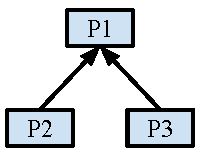
\includegraphics[width=\linewidth]{Individuals.pdf}
\caption{When processes are alone they will join the group with $\Pr=p^8$} \label{fig:groupinga}
\end{subfigure}
\hspace*{\fill} % separation between the subfigures
\begin{subfigure}{0.45\textwidth}
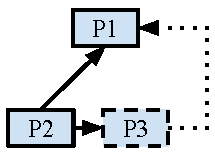
\includegraphics[width=\linewidth]{ForwardedInvites.pdf}
\caption{As a member of P2's group, P3 has a $\Pr=p^6$ of joining P1's group.} \label{fig:groupingb}
\end{subfigure}
\caption{The grouping processes effects the outcome of elections} \label{fig:grouping}
\end{figure}

Figure \ref{fig:grouping}, shows an example of how the grouping of the processes would affect the distribution of election outcomes.
To the considered process ($P$), the probability of transitioning to a given observed group size would depend on the grouping of other processes in the system.
In order to be able to predict this information, the considered process would need either complete information of the state of the system or would need to predict what state the system is in probabilistically.
A probabilistic prediction would depend on how long the processes have been separated.
After a long enough period of time the distribution of states for the processes could be found using a steady-state analysis.
However, when processes uses $Recovery()$ they are deterministically placed in the alone state.
As a consequence the state of the system depends on the number of steps since the last reconfiguration, which violates the memoryless property.

In Figure \ref{fig:grouping}, the probability of grouping depends on the state of the processes.
Suppose P1 fails to detect P2 and P3 multiple times.
The probability P2 has grouped with P3 could then be modeled as a two process sub-case of this 3 process case.
Let this two process sub-case be described with a profile chain $P_{sub}$.
The probability of P2 and P3 joining P1's group depends on the state of the sub-case.
Additionally the probability distribution of an observation of the sub-case depends how many steps the sub-case has completed.
If $P_{sub}$ is ergodic, then $Steady(P_{sub}{}) \neq [1.0 \quad 0]$.
Each step of the sub-case ($n$) will move its distribution asymptotically closer to the steady-state:
 
\[ [1.0 \quad 0] * \lim_{n \to \infty}P_{sub}^n = Steady(P_{sub}) \]  

Since the initial state of the algorithm in the sub-case must be un-grouped ($[1.0 \quad 0]$), and the process is ergodic, the probability distribution of the sub-case depends on the number of steps ($n$).
As a consequence, the distribution for any $n$ must be different from the distribution of $n-1$. 
Since the probability of P1 completing an election of P2 and P3 depends on the grouping of P2 and P3, the behavior of the full case cannot be memoryless, since it is a function of $n$.
In particular, it would need a Markov chain of sufficient order to capture this phenomena with a small enough amount of error.
Therefore, to make the algorithm memoryless, only a selected process may lead a multiprocess group.

\subsection{Ready Acknowledgment}

The changes added a third message to completing an election -- a ready acknowledge message.
This message is sent by a member after receiving the ready message from the coordinator.
This allows the coordinator to be certain of the member's status before the next round.
Without the ready acknowledgment, the member may not receive the ready message and the coordinator will observe the member is a part of the group.
This interaction is shown in Figure \ref{fig:lostready}.

\begin{figure}
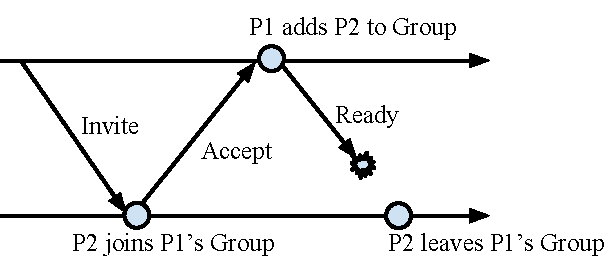
\includegraphics[width=\linewidth]{LostReady.pdf}
\caption{The grouping processes effects the outcome of elections} \label{fig:lostready}
\end{figure}

As a consequence, the probability a member remains in a group in the first round after an election has a different probability than each subsequent round.
Since the loss of the ready message changes the member's state and not the leader's state, the probability P1 stays in a group with P2 depends on the ready message and the exchange of the ``Are You Coordinator'' message.
By adding the extra message, the observation of the coordinator must be the state of the member of the group.
As a consequence, the probability a member remains in a group in the first round after an election is identical to each subsequent round.

\subsection{Failure Detection}

Members cannot leave a group without the leader's permission.
Members do not suspect the coordinator has failed, only the coordinator may suspect the members.
For the purpose of starting an election, an ``Are You There'' message and its negative response are considered equivalent to a ``Are You Coordinator'' message and a positive response.
On receipt of the negative response, the member will immediately recover and become a leader.
This assumption relies on ``Are You Coordinator'' and ``Are You There'' messages being sent at roughly the same time.

This change leads to a live-lock situation in a crash failure, where the group's leader crashes and does not return and as a consequence the remaining members are trapped in a group without a leader.
For the purpose of this work, we have disregarded these live lock scenarios.
However, the live-lock could be avoided if the member can detect it has not received an ``Are You Coordinator'' message in a round.
When the process fails to receive the message, the coordinator must have also removed the member from their group since they could not have received an ``Are You Coordinator'' response message.
Integrating this component is an area of future work.

\subsection{Creation of A Profile Chain}

The election algorithm produces and distributes a set of processes $UpPeers$ and a coordinator of that set.
$UpPeers$ is distributed via message passing and maintained by the coordinator.
Different processes may have different versions of $UpPeers$ for a given coordinator as processes enter and leave the group.
However, a process will eventually receive an up-to-date version of $UpPeers$ from the coordinator, or it will leave the group.

To model the behavior of the algorithm, at each time-step the selected process recorded the cardinality of its membership set $UpPeers$.
The selected process was always the coordinator of any formed group, and was the only process that could lead a multi-process group.
The cardinality of $UpPeers$ directly mapped to the state in the Markov Chain.
For example given the membership set $S=\{P1,P2,P3\}$, then $\left | S \right |=3$ and the state of the system in the Markov chain is also $i=3$.

The profile Markov chain for the algorithm was constructed as a closed form representation of the algorithm's behavior.
In a distributed system, information about what other processes consider to be their state cannot be easily known.
Therefore, a model should only consider the effects a process could locally observe.
The chain models the observations of a single process.
The process can only observe what it considers its local group.

Each round, the behavior is described by two components: maintaining a group that already exists, and inviting other processes into the group.
The coordinator will exchange a ``Are You Coordinator'' message and the peer will respond to verify is still available.
To maintain a group of $m$ other processes, the probability is defined as a random variable with the following probability distribution (pdf):

\[
 \Pr_{M}(X=k; m) = 
   \begin{cases}
    \binom{m}{k} p^{2k}(1-p^2)^{m-k} & \quad \text{if } 0 \leq k \leq m \\
    0                                & \quad \text{otherwise} \\
  \end{cases}
\]

Where $k$ is the number of processes remaining in a group selected from $m$ processes.
A process will leave a group if, from the considered process' perspective, they do not respond to an ``Are You Coordinator'' message.
A process cannot leave a group without the coordinator's permission: other processes cannot change their state without coordinating with the leader.

To invite other processes to the group, the two processes ultimately exchange up to 8 messages.
In a round, a single process can invite many other processes to its group.
From a selection of $n$ other coordinators, the probability distribution for joining a new group with $k$ of the $n$ processes is:

\[
	\Pr_{I}(Y=k; n) =
	\begin{cases}
		\binom{n}{k} p^{8k}(1-p^8)^{n-k} & \quad \text{if } 0 \leq k \leq n \\
		0                                & \quad \text{otherwise} \\
	\end{cases}
\]

In the profile chain, in a state $s$ that describes the number of processes in a group, the probability of transitioning from $s$ to $s'$ with $n$ total processes (including the considered process) is:

\[ \Pr_{T}(Z=s'; n; s) = \sum_{i=0}^{s-1} \sum_{j=0}^{s'-i-1} \Pr_{M}(X=i; s-1) \Pr_{I}(X=j; n-s-1) \]

From this distribution, a set of transition probabilities can be calculated for a given omission rate $p$ and number of processes $n$.
This set of transition probabilities forms a profile Markov chain $P$, which can be evaluated to for any number of processes $n$ and omission rate $p$.
The generated profile chain is ergodic when $0<p<1.0$. The profile chain is a stationary Markov chain.


